\subsection{Schnittstellenbeschreibungen}
Das folgende Kontextdiagramm (Abbildung \ref{fig:kontextdiagramm}) zeigt eine Übersicht über das System und sämtlichen Schnittstellen. In den folgenden Abschnitten werden die Schnittstellen im Detail beschrieben.

\begin{figure}[h!]
	\centering
	\includegraphics[width=0.9\linewidth]{../../fig/kontextdiagramm}
	\caption{Kontextdiagramm}
	\label{fig:kontextdiagramm}
\end{figure}

Die Schnittstellen Start Signal, Stop Signal und Camera Config werden von einem Webserver als REST\footnote{Representational State Transfer}-Ressourcen zur Verfügung gestellt. Dadurch wird der Aufrufer nicht auf eine bestimmte Programmiersprache beschränkt. Zudem können die Schnittstellen in der Testphase mit einem einfachen Browser angesteuert werden.

TODO REST-Schnittstelle des Start Signals beschreiben

\subsubsection{Stop Signal}
Die Schnittstelle Stop Signal wird vom Webserver auf der externen Steuereinheit angeboten. Die Adresse von diesem Webserver ist dem Raspberry Pi, durch das Start Signal, bekannt. Wenn das Programm auf dem Raspberry Pi beendet ist schickt es einen PUT-Request an den Webserver auf der externen Steuereinheit und signalisiert so das Stop Signal. Tabelle \ref{tab:put-stop-signal} zeigt ein Beispiel der Anfrage.

\begin{table}[h!]
	\centering
	\begin{tabular}{|l|l|}
		\hline Anfrage an externe Steuereinheit	 & Antwort von externer Steuereinheit \\ 
		\hline \verb|PUT /stop-signal HTTP/1.1|  & \verb|200 OK| 					  \\
			   \verb|Host: 192.168.1.3| 		 & 							          \\
		\hline 
	\end{tabular} 
	\caption{PUT-Request an Stop Signal}
	\label{tab:put-stop-signal}
\end{table}

Durch dieses Design muss die externe Steuereinheit nicht permanent nach dem Status des Programms fragen (Polling). Der Webserver auf der externen Steuereinheit verarbeitet den Request und gibt das Stop Signal visuell aus.

\newpage

TODO REST-Schnittstelle der Camera Config beschreiben

\newpage

\subsubsection{raspistill}
\label{subsub:raspistill}
Die Kamera wird über das mitgelieferte Kommandozeilenprogramm \verb|raspistill| angesteuert. Das Programm bietet zahlreiche Einstellungsmöglichkeiten. Eine kleine, für das Projekt relevante Auswahl ist in der Tabelle \ref{tab:raspistill} aufgeführt. Eine ausführliche Dokumentation des Programms kann man unter folgendem Link abrufen: \\

\href{http://www.raspberrypi.org/wp-content/uploads/2013/07/RaspiCam-Documentation.pdf}{http://www.raspberrypi.org/wp-content/uploads/2013/07/RaspiCam-Documentation.pdf} \\

\begin{table}[h!]
	\renewcommand{\arraystretch}{1.5}
	\begin{tabular}{|l|p{14cm}|}
		\hline Option & Beschreibung \\ 
		\hline \verb|--nopreview| & Deaktiviert die Bildvorschau (Optimierung) \\ 
		\hline  \verb|--quality 50| & Tests haben gezeigt, dass die Qualität von 50 genügt. Die Bildgrösse wird somit einiges kleiner. \\ 
		\hline  \verb|--roi| & Bildausschnitt festlegen \\ 
		\hline  \verb|--contrast| & Kontrast einstellen \\ 
		\hline  \verb|-cfk 128:128| & Erzeugt ein Bild in Graustufen \\ 
		\hline 
	\end{tabular} 
	\caption{Relevante Einstellungen von raspistill}
	\label{tab:raspistill}
\end{table}

Ein Aufruf von \verb|raspistill| könnte wie folgt aussehen (wird in diesem Projekt nicht verwendet): \\

\verb|raspistill --nopreview --quality 50 -roi 0.5,0.5,0.25,0.25 --contrast 50 -cfx 128:128| \\

Das Programm speichert das Bild anschliessend in einer jpg-Datei ab. Für die weitere Verarbeitung des Bildes ist das nicht optimal. Das Bild müsste vom Python-Programm, welches für die Erkennung des Korbes zuständig ist, nochmals eingelesen werden. Deshalb wird \verb|raspistill| direkt aus dem Erkennungs-Programm über ein Python-Interface angesteuert. Dieses Interface wird von der Bibliothek \verb|picamera|\footnote{\href{http://picamera.readthedocs.org/en/release-1.8/index.html}{http://picamera.readthedocs.org/en/release-1.8/index.html}} zur Verfügung gestellt und ermöglicht ein Objekt der Kamera zu erstellen. Das Kamera-Objekt liefert direkt ein Bild als PIL\footnote{Python Image Library}-Objekt zurück. Das PIL-Objekt kann anschliessend für die weitere Verarbeitung in Python genutzt werden. Auflistung \ref{lst:picamera} zeigt ein Codeausschnitt wie die Kamera in diesem Projekt angesteuert wird.

\begin{lstlisting}[language=Python,caption={Bild aufnehmen mit der Raspberry Pi Camera},label=lst:picamera]
import io
import time
import picamera
from PIL import Image

# Create the in-memory stream
stream = io.BytesIO()
with picamera.PiCamera() as camera:
camera.start_preview()
time.sleep(2)
camera.capture(stream, format='jpeg')
# "Rewind" the stream to the beginning so we can read its content
stream.seek(0)
image = Image.open(stream)
\end{lstlisting}


\subsubsection{UART}
\label{subsub:uart}
Die UART Schnittstelle dient der Kommunikation zwischen dem Raspberry Pi und dem Freedomboard, welches die LowLevel Funktionalität der Maschine umsetzt. Dieses implementiert sämtliche Ansteuerungen von Hardwarekomponenten wie Motorentreibern oder Sensoren. Die übergeordnete Instanz des Freedomboards ist der Raspberry Pi, welches die Schnittstelle zum Benutzer bildet. 
Die für diese Abstraktion notwendige Schnittstelle wird mittels UART
implementiert. UART\footnote{Universal Asynchronous Receiver Transmitter}
ist ein weit verbreiteter Standard für serielle Schnittstellen. Ein mögliches
Protokoll ist in der Tabelle \ref{tab:uart}
zusammengefasst. Optionale Parameter sind dabei in eckige Klammern gesetzt.
Die erlaubt es einfachere Automaten bzw. Statemachines zu erstellen, da das
setzen und auslesen von Parametern mit den selben Kommandos erfolgt.

Die serielle Schnittstelle wird vom Freedomboard direkt implementiert auf
USB mittels einer USB-Seriell Wandlung. Dies ermöglicht es, das Freedomboard
direkt per USB-Kabel am Raspberry Pi zu verbinden.

\begin{table}[h!]
	\centering
	\begin{tabular}{l l l l l}
		Aktion & Message & Parameter & Antwort \\
		\hline
		drehen um $\varphi$ 
			& \verb!rotate!
			& [Winkel $\varphi$]
			& aktuelle Position \\
		Entfernung $s$ setzen
			& \verb!distance!
			& [Entfernung $s$]
			& aktuelle Entfernung \\
		Ausrichtungsmotor enable
			& \verb!rotater!
			& [enable/disable]
			& aktueller Status \\
		Schussmotor enable
			& \verb!shooter! 
			& [enable/disable]
			& aktueller Status \\
		Lademotor enable
			& \verb!loader!
			& [enable/disable]
			& aktueller Status \\
		Schussmotor einstellen
			& \verb!setrpm!
			& [RPM]
			& aktueller Status \\
		Schussabgabe
			& \verb!fire!
			& -
			& ok/nok \\
		Reset
			& \verb!reset!
			& -
			& -\\
	\end{tabular}
	\caption{Protokollentwurf der seriellen Schnittstelle}
	\label{tab:uart}
\end{table}

Für die Entwicklungsphase sind zu den in der Tabelle \ref{tab:uart}
aufgeführten Kommandos noch weitere zu implementieren. Beispielsweise
ist es nützlich, einige Maxima und Minima für allfällige
Reglerparametrierungen abrufen zu können. Ein Beispiel hierfür ist das
Anfahren und Zurückstellen des Schussmotors wie in der Abbildung
\ref{fig:shooter} dargestellt.

\begin{figure}[h!]
	\centering
	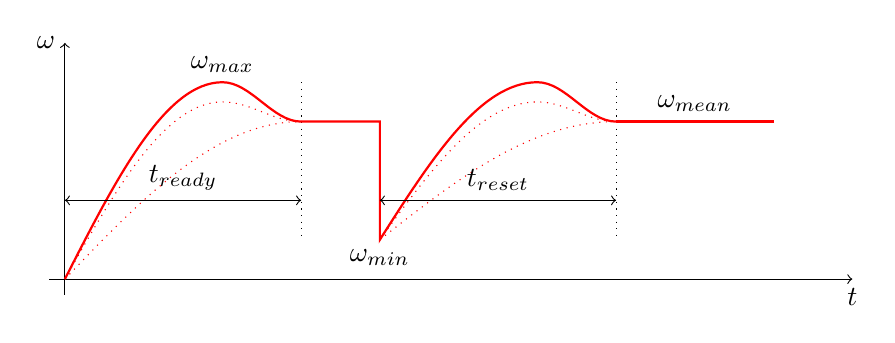
\begin{tikzpicture}
		% Koordinaten
		\draw[->] (-0.2,0) -- (10,0) node[anchor=north] {$t$};
		\draw[->] (0,-0.2) -- (0,3) node[anchor=east] {$\omega$};
		% Hilfslinien
		\draw[dotted] (3,2.5) -- (3,0.5);
		\draw[dotted] (7,2.5) -- (7,0.5);
		% Kurve - Anfahren
		\draw[red, thick] 
			(0,0) sin (2,2.5) cos (2.5,2.25) sin (3,2);
		\draw[red, dotted]
			(0,0) sin (2,2.25) cos (2.5,2.125) sin (3,2);
		\draw[red, dotted]
			(0,0) sin (3,2);
		% Kurve - Einbruch
		\draw[red, thick] 
			(3,2) -- (4,2) -- 
			(4,0.5) sin (6,2.5) cos (6.5,2.25) sin (7,2);
		\draw[red, dotted]
			(4,0.5) sin (6,2.25) cos (6.5,2.125) sin (7,2);
		\draw[red, dotted]
			(4,0.5) sin (7,2);
		% Kurve - Ende
		\draw[red, thick] (7,2) -- (9,2);
		% Markierungen
		\draw[] (2,2.5) node[anchor=south] {$\omega_{max}$};
		\draw[] (4,0.5) node[anchor=north] {$\omega_{min}$};
		%\draw[] (4,3) node[anchor=south] {Schuss};
		\draw[] (8,2) node[anchor=south] {$\omega_{mean}$};
		% Zeiten
		\draw[<->] (0,1) -- (3,1) node[midway, above] {$t_{ready}$};
		\draw[<->] (4,1) -- (7,1) node[midway, above] {$t_{reset}$};
	\end{tikzpicture}
	\caption{Vereinfachter Verlauf der Schussmotorendrehzahl für Anfahrt
		und einfache Schussabgabe}
	\label{fig:shooter}
\end{figure}

\newpage
\subsubsection{LowLevel}
Als LowLevel Schnittstellen werden die einfachen Ansteuerungen
bezeichnet, welche direkt mittels eines Mikrocontroller erzeugt
werden.

Die einzelnen Hardwarekomponenten wie Motorentreiber werden mittels
einfachen digitalen Signalen bedient. Dies können einfache digitale
Pegel sein, standardisierte Busse wie I$^2$C oder spezielle Signale
wie PWM\footnote{Pulsweitenmodulation}. 

Da noch nicht alle Hardwarekomponenten definiert sind, gibt es keine
definitive Aussage über die verwendeten Signale bzw. Busse. Vorzusehen
sind sicherlich I$^2$C und SPI, da diese weit verbreitete Schnittstellen
sind, durch das Freedomboard unterstützt werden und deren
Implementierung relativ einfach ist.


